\section{Results}
\subsection{Matched correction of a developed driven front}
At $\eta=0.1W$, $h=0.005W$ and $\Dt_{\rm raw}=10^{-7}$, the native and corrected calculations share the physical matrices, stencil, projection, initial field and relative horizon. Their sole force-law difference is Eq.~\eqref{eq:corrected}. Migration-speed error falls from 16.014\% to 0.452\%, and terminal aligned RMS error from $0.105147W$ to $0.006016W$ (Fig.~\ref{fig:n20}). These are approximately 97.2\% and 94.3\% error reductions within this matched comparison.

The shape improvement extends over the profile and does not result from fitting its translation speed: both reconstructed shapes receive the same alignment operation. Both routes meet the retained settling and invariant criteria. Because they start from a common developed field, this test isolates the evolution correction but does not establish cold-start performance or supply its initialization for free in an end-to-end cost comparison.

\begin{figure}[tbp]
 \centering
 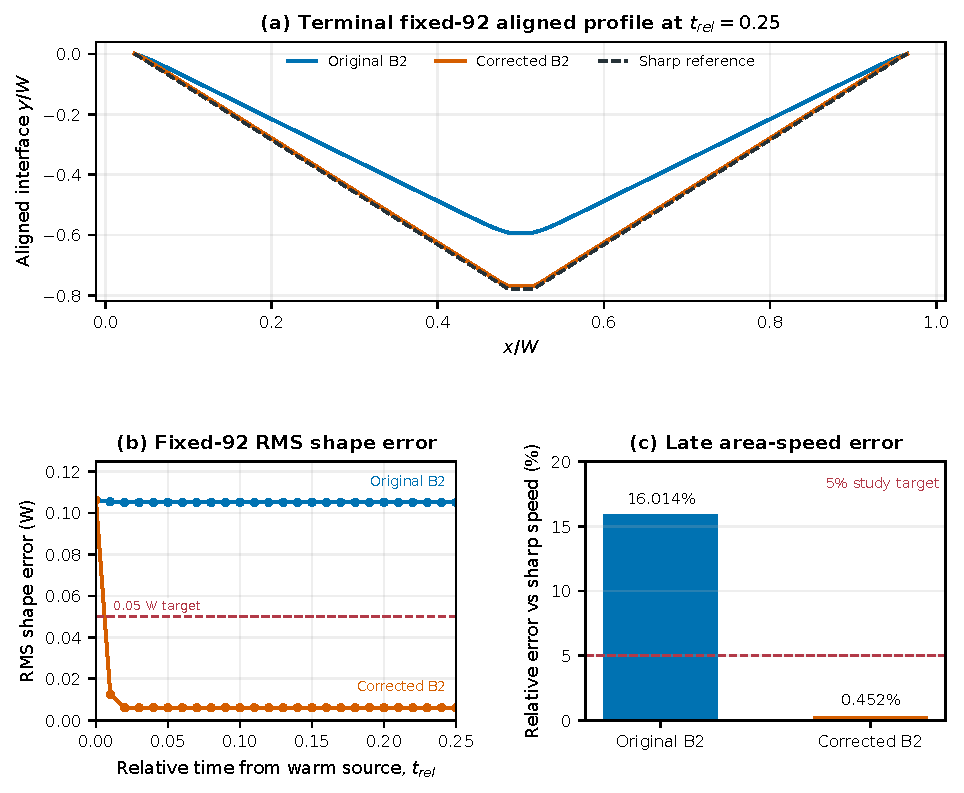
\includegraphics[width=\linewidth]{fig01_n20_matched.pdf}
 \caption{Matched translating-front comparison. Terminal profiles are maximum-aligned, and the dashed curve in panel (a) is the retained sharp reference. The shape history uses the fixed 92-point RMS definition. Time is elapsed time from the common developed state. The speed comparison uses the same sharp target. Both routes use $\eta=0.1W$, $h=0.005W$ and $\Dt_{\rm raw}=10^{-7}$.}
 \label{fig:n20}
\end{figure}

\subsection{Cold starts and a thinner conventional calculation}
A separate comparison starts each route from its width-specific compact profile and includes binary calibration. The corrected recipe uses $\eta=0.1W$, $h=0.01W$ and $\Dt_{\rm raw}=4\times10^{-7}$. The thinner conventional recipe uses $\eta=0.02W$, $h=0.005W$ and $\Dt_{\rm raw}=1.25\times10^{-6}$. The corrected route gives terminal aligned RMS error $0.004087W$ and speed error 1.326\%, compared with $0.013686W$ and 4.596\% for the selected thinner route.

Recorded end-to-end wall times, including calibration, are approximately 1035 and 1047~s. This pair therefore demonstrates better accuracy at a similar observed cost despite the wider interface and coarser grid. It does not isolate an intrinsic multiplier speedup: width, grid and timestep differ, and the observations are single realizations rather than an optimized accuracy--cost frontier.

\subsection{Interacting junctions and local memory}
\label{sec:interactions}
The cold interacting-junction test compares native, whole-correction and local-memory routes at the same $\eta=0.08W$, $h=0.01W$, nine-point Laplacian, raw timestep $4\times10^{-7}$, clock factor and initial field. Figure~\ref{fig:h24} and Table~\ref{tab:h24} show the largest sampled absolute shape errors.

\begin{table}[pos=htbp,abovecap=10pt]
\caption{Matched cold interacting-junction comparison. Entries are maximum sampled Hausdorff errors divided by $W$, distinct from the aligned RMS metric of Fig.~\ref{fig:n20}.}
\label{tab:h24}
\centering
\begin{tabular}{lrr}
\toprule
Method & Short pair & Long pair\\
\midrule
Native B2, nine-point stencil & 0.10609 & 0.14075\\
Whole spatial correction & 0.02694 & 0.03058\\
Spatial correction with local memory & 0.01399 & 0.01814\\
\bottomrule
\end{tabular}
\end{table}

The whole correction brings all sampled shapes below $0.05W$. Local memory supplies a further reduction of approximately 48.1\% and 40.7\% in the two worst sampled errors, with identical disappearance-time brackets for the two corrected routes. Memory thus supplies additional shape margin rather than being necessary to meet the selected tolerance.

At doubled raw timestep $8\times10^{-7}$, separately completed whole and local calculations retain worst errors $0.02696W/0.03064W$ and $0.01404W/0.01820W$. Both meet speed, disappearance-time and sampled-shape targets. Recorded peak resident memory is approximately 459 and 912~MB, respectively. Wall times were measured in different execution contexts and do not isolate controller overhead.

Other controls limit the interpretation. At $\eta=0.12W$, persistent memory improves two postinteraction shape samples by approximately 39\% and 13\% relative to a cadence-reset variant, although both variants meet $0.05W$. In an asymmetric interaction, whole and local routes give worst errors $0.01586W$ and $0.01437W$; the local route costs more in that sequential comparison. These observations support a case-dependent history benefit, not a requirement for memory whenever junctions interact.

\begin{figure}[tbp]
 \centering
 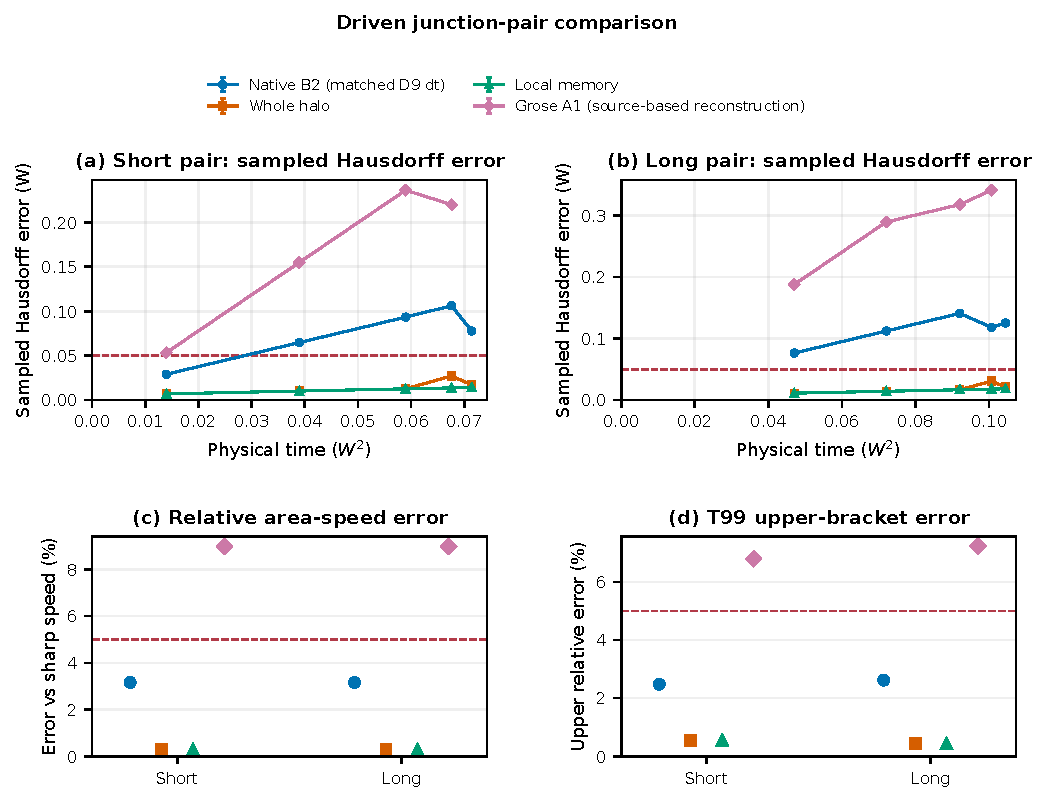
\includegraphics[width=\linewidth]{fig02_h24_routes_grose.pdf}
 \caption{Driven grain-consumption comparisons. The native, whole-correction and local-memory B2 routes share the cold initial field, width, grid, nine-point stencil and raw timestep. The Grose--Asimow reconstruction is a distinct source-based formulation at the same width and grid, with its own binary clock and numerical ingredients. Its selected recipe is compared, not the entire method's attainable performance. The fifth reconstructed-method shape observation for each pair has an empty boundary and therefore no finite ordinate.}
 \label{fig:h24}
\end{figure}

\subsection{A reconstructed high-driving-force method}
Grose--Asimow \citep{grose2022} is the closest conceptual comparator because it directly treats large driving forces at multiphase junctions. We reconstructed its force allocation, recursive transfer, finite-difference correction and grouped profile-restoration procedure. The operative pair equations are used where a printed segregation-sign expression conflicts with them. The numerical conventions needed for profile-anchor tracing and simultaneous events are documented in the Supplementary Material.

At the interacting-case width and grid, the declared amplification settings $A_\sigma=0$ and 1 do not meet the joint shape-and-kinetics targets. For the selected $A_\sigma=1$ half-step control, migration speed remains approximately 8.98\% above the sharp reference. Eight finite shape samples exceed $0.05W$, and two late boundaries are absent. Halving the timestep changes fitted speed by approximately 0.069\%, while shape discrepancies persist.

This compares specified independent implementations on a new driven unequal-energy interaction geometry. It is not a reproduction of the authors' executable or every published figure, nor an optimization of the free amplification parameter. The result supports an accuracy advantage over these reconstructed recipes on the present outputs. It does not establish failure of the published method in general or a speedup over its optimized implementation.

\subsection{Sensitivity to strength and radius}
\label{sec:robustness}
Four one-factor perturbations test the prescription $\chi=27$, $\rho=\eta$ in the developed-front case with $\eta=0.1W$ and $h=0.01W$. Strengths 20 and 34 are tested at radius ten cells; radii eight and twelve cells are tested at strength 27. The outcomes do not select a replacement baseline.

All four cases meet the retained speed, shape, settling and invariant criteria. Migration-speed errors range from approximately 1.07\% to 1.30\%, and terminal aligned RMS errors from $0.00366W$ to $0.00472W$ (Fig.~\ref{fig:robustness}). Thus the benefit is not restricted to one isolated parameter value in this case. These points do not define a continuous admissible region or an automatic parameter rule.

\begin{figure}[tbp]
 \centering
 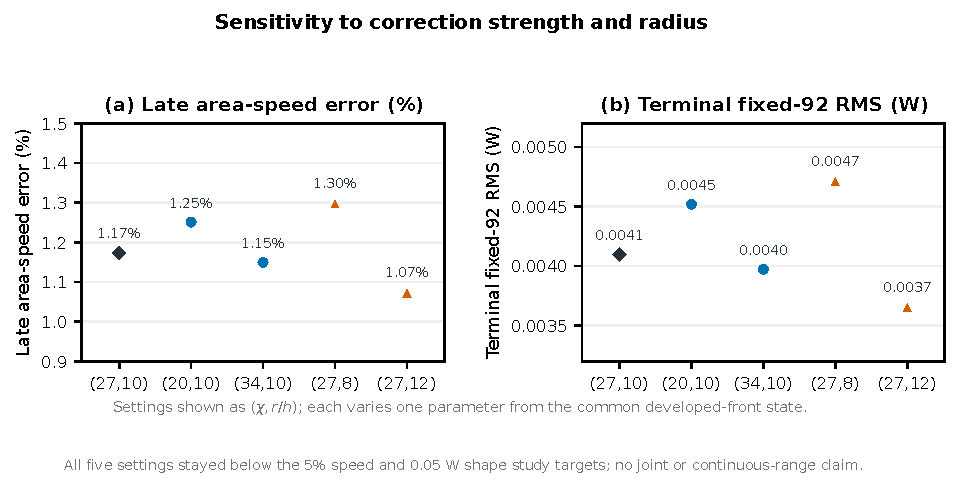
\includegraphics[width=\linewidth]{fig03_parameter_robustness.pdf}
 \caption{One-factor sensitivity around $\chi=27$ and $\rho/h=10$ in the developed-front benchmark. Strength and radius are perturbed separately. Points represent completed prescribed calculations, not a fitted parameter-response surface.}
 \label{fig:robustness}
\end{figure}

\subsection{Transfer to OpenPhase}
\label{sec:openphase}
We inserted the whole spatial correction into OpenPhase Academic \citep{tegeler2017}, using the pinned source revision specified in Ref.~\citep{openphase}. OpenPhase has its own local phase storage, pair assembly, driving-force merge and increment normalization. Only existing antisymmetric capillary increments are scaled, after native capillary calculation and before bulk-force merging. These operations are not replaced by our B2 kernel or Euclidean projector. The fixed prescription remains $\chi=27$, $\rho=\eta=0.08W$, giving eight cells at $h=0.01W$. The raw timestep remains $10^{-6}$.

Cold native and corrected trajectories share the initial field, boundaries, schedule, binary clock and $0.12$ horizon. Migration-speed error decreases from 25.532\% to 0.983\%. Short-pair $T_{99}$ error falls from a 15.736--16.031\% bracket to 0.787--1.084\%; the long-pair bracket falls from 17.226--17.430\% to 0.784--0.992\%.

Shape improvement is substantial but incomplete (Fig.~\ref{fig:openphase}). All five short-pair samples meet $0.05W$, with largest sampled error $0.04570W$. Four of five long-pair samples meet that target. At $t=0.10068814$, the remaining sample has error $0.05862W$ and sampling bracket $[0.05857W,0.05867W]$, entirely above the target. The next sample gives $0.04826W$. The fixed correction therefore improves this second implementation without refitting but does not remove every late shape discrepancy.

A fixed-grid, two-level timestep check repeats the same cold OpenPhase initial field and prescription at raw step $5\times10^{-7}$ to the same physical horizon, with a separately calibrated binary clock. The signed speed errors are $-25.595\%$ (native) and $-0.982\%$ (whole correction), close to $-25.532\%$ and $-0.983\%$ at $10^{-6}$. Corrected short- and long-pair $T_{99}$ errors remain within 5\% (0.787--1.085\% and 0.785--0.993\%); the corrected shape outcomes are again five of five short-pair passes and four of five long-pair passes. The late long-pair sample remains above $0.05W$ at $0.05859W$, including its sampling bracket. This is a two-level fixed-grid sensitivity check, not an asymptotic convergence study; detailed readouts are in Supplementary Table~S2.

Saved preinteraction fields also permit fixed-window fits of outer interface profiles away from the ternary diffuse core and correction support. In B2, the fitted two-arm included angle changes from 72.835--72.842$^\circ$ (native) to 60.093--60.094$^\circ$ (corrected), against a same-window sharp value of $60^\circ$. In OpenPhase, the corresponding descriptive upper/lower profile-corner angle changes from 63.918--63.925$^\circ$ to 82.251--82.480$^\circ$, against same-window sharp values of 82.819--82.997$^\circ$. These are outer-profile descriptors, not core selection angles. The native signed speed errors have opposite signs in the two implementations (+16.014\% in B2 and $-25.532\%$ in OpenPhase), so the geometric response does not establish a common positive-drag mechanism. Fit windows and definitions are given in Supplementary Table~S3.

\begin{figure}[tbp]
 \centering
 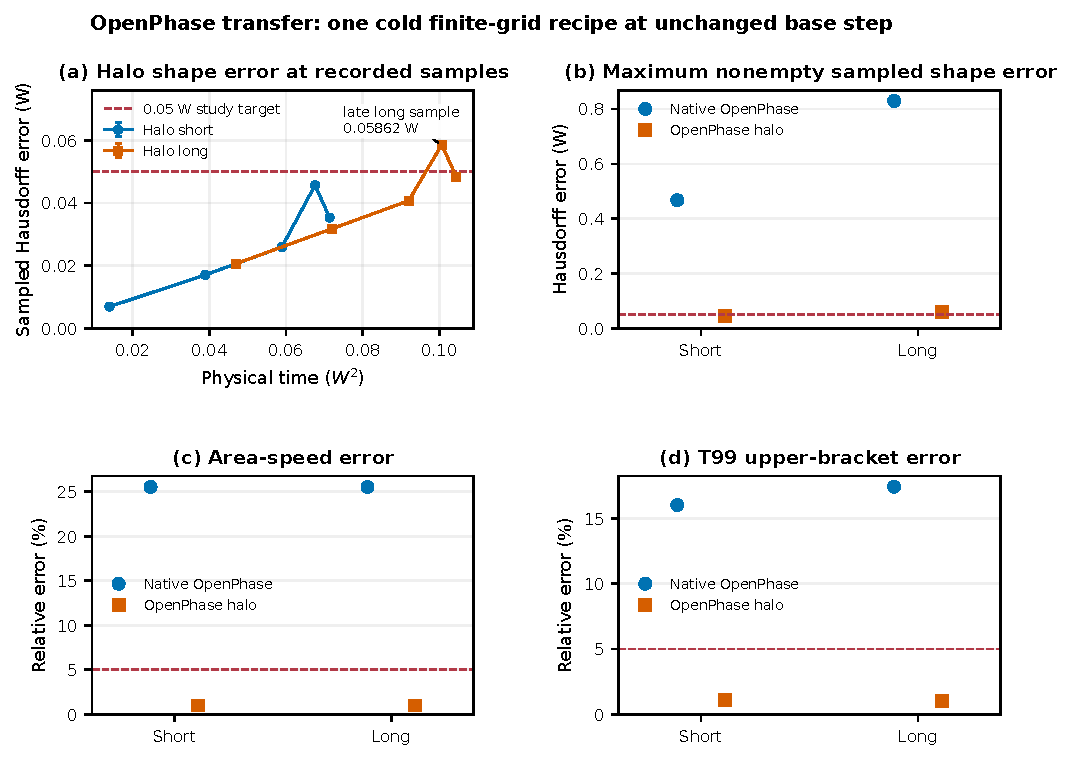
\includegraphics[width=\linewidth]{fig04_openphase_transfer.pdf}
 \caption{Fixed-prescription transfer to OpenPhase. Shape distances use actual saved physical times and the same sharp-reference construction. The long-pair sample above $0.05W$ is retained. Maxima in panel (b) include only nonempty boundaries; native empty-boundary observations are additional failures rather than zero distances. Passing migration-speed and disappearance-time targets does not imply accurate morphology at every sampled time.}
 \label{fig:openphase}
\end{figure}
